\section{Model matematyczny lewitacji magnetycznej}

Do zastosowania algorytmu sterowania QTO-RHC niezbędny jest model układu. Decyzja o sterowaniu podejmowana jest na podstawie rozwiązań równań układu i równań sprzężonych. Stanowisko laboratoryjne magnetycznej lewitacji przedstawia rysunek \ref{rys:maglev}.

\begin{figure}[!htb]
  \begin{center}
    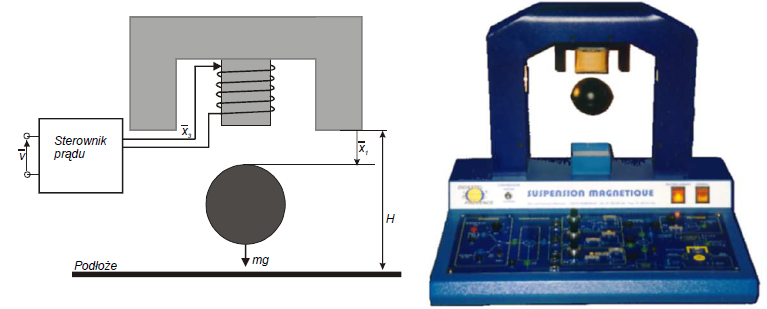
\includegraphics[scale=0.85]{img/maglev.PNG}
    \caption{Stanowisko laboratoryjne magnetycznej lewitacji}
  \end{center}
  
  \label{rys:maglev}
\end{figure}

Równania różniczkowe układu, po przeskalowaniu skalowania, zmiennych stanu oraz czasu:

\begin{equation}
  \begin{cases}
    \dot{x}_1 & = x_2 \\
    \dot{x}_2 & = -e^{-x_1} \cdot x_3^2 + 1 \\
    \dot{x}_3 & = -cx_3 + u
    \end{cases}
\end{equation}

Zastosowane przeskalowanie:
\begin{equation}
\bar{x}_1 = \alpha x_1,
\bar{x}_2 = \beta x_2,
\bar{x}_3 = \gamma x_3,
\bar{\nu} = \frac{\eta u \tau + I i_s}{k},
\bar{\tau} = \xi t
\end{equation}

Gdzie $\bar{x}_1 [m]$ oznacza odległość kuli od elektromagnesu, $\bar{x}_2 [m/s]$ jej prędkość,  $\bar{x}_3 [A]$ prąd cewki elektromagnesu oraz $\bar{\nu} [V]$ napięcie sterujące. Pełne wyprowadzenie modelu można znaleźć w pracy dyplomowej \cite{Bania1999}.
 
Współczynniki przeskalowania zebrano w tabeli.

\begin{table}[!htb]
  \centering
  \begin{tabular}{|c|l|l|}
  \hline
  Współczynnik & Wartość \\
  \hline
  $\alpha$ & $0,00773746 m$ \\
  \hline
  $\beta$ & $0,275507681 m/s$ \\
  \hline
  $\gamma$ & $0,28890446065998 A$ \\
  \hline
  $\xi$ & $0,2808437120924$ \\
  \hline
  $\eta$ & $10,28701901522286 A/s$ \\
  \hline
  \end{tabular}
  \caption{Parametry przeskalowania modelu}
  \label{tab:idf}
\end{table}


